\colorlet{ind}{black}
\colorlet{dep}{gray!50!white}
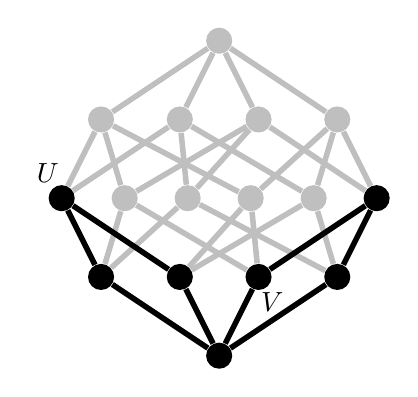
\begin{tikzpicture}
  \draw (0, 4)    node[circle, fill, color=dep] (abcd) {};
  \draw (-1.5, 3) node[circle, fill, color=dep] (abc) {};
  \draw (-0.5, 3) node[circle, fill, color=dep] (abd) {};
  \draw (+0.5, 3) node[circle, fill, color=dep] (acd) {};
  \draw (+1.5, 3) node[circle, fill, color=dep] (bcd) {};
  \draw (-2.0, 2) node[circle, fill, color=ind] (ab) {};
  \draw (-1.2, 2) node[circle, fill, color=dep] (ac) {};
  \draw (-0.4, 2) node[circle, fill, color=dep] (ad) {};
  \draw (+0.4, 2) node[circle, fill, color=dep] (bc) {};
  \draw (+1.2, 2) node[circle, fill, color=dep] (bd) {};
  \draw (+2.0, 2) node[circle, fill, color=ind] (cd) {};
  \draw (-1.5, 1) node[circle, fill, color=ind] (a) {};
  \draw (-0.5, 1) node[circle, fill, color=ind] (b) {};
  \draw (+0.5, 1) node[circle, fill, color=ind] (c) {};
  \draw (+1.5, 1) node[circle, fill, color=ind] (d) {};
  \draw (0, 0)    node[circle, fill, color=ind] (o) {};
  \draw[line width=2pt, color=dep] (abcd) -- (bcd);
  \draw[line width=2pt, color=dep] (abcd) -- (acd);
  \draw[line width=2pt, color=dep] (abcd) -- (abd);
  \draw[line width=2pt, color=dep] (abcd) -- (abc);
  \draw[line width=2pt, color=dep] (bcd) -- (cd);
  \draw[line width=2pt, color=dep] (bcd) -- (bd);
  \draw[line width=2pt, color=dep] (bcd) -- (bc);
  \draw[line width=2pt, color=dep] (acd) -- (cd);
  \draw[line width=2pt, color=dep] (acd) -- (ad);
  \draw[line width=2pt, color=dep] (acd) -- (ac);
  \draw[line width=2pt, color=dep] (abd) -- (bd);
  \draw[line width=2pt, color=dep] (abd) -- (ad);
  \draw[line width=2pt, color=dep] (abd) -- (ab);
  \draw[line width=2pt, color=dep] (abc) -- (ab);
  \draw[line width=2pt, color=dep] (abc) -- (ac);
  \draw[line width=2pt, color=dep] (abc) -- (bc);
  \draw[line width=2pt, color=dep] (ac) -- (a);
  \draw[line width=2pt, color=dep] (ac) -- (c);
  \draw[line width=2pt, color=dep] (ad) -- (a);
  \draw[line width=2pt, color=dep] (ad) -- (d);
  \draw[line width=2pt, color=dep] (bc) -- (b);
  \draw[line width=2pt, color=dep] (bc) -- (c);
  \draw[line width=2pt, color=dep] (bd) -- (b);
  \draw[line width=2pt, color=dep] (bd) -- (d);
  \draw[line width=2pt, color=ind] (ab) -- (a);
  \draw[line width=2pt, color=ind] (ab) -- (b);
  \draw[line width=2pt, color=ind] (cd) -- (c);
  \draw[line width=2pt, color=ind] (cd) -- (d);
  \draw[line width=2pt, color=ind] (a) -- (o);
  \draw[line width=2pt, color=ind] (b) -- (o);
  \draw[line width=2pt, color=ind] (c) -- (o);
  \draw[line width=2pt, color=ind] (d) -- (o);
  \draw (c)  node[right=5pt, below=2pt] {$V$};
  \draw (ab) node[left=5pt, above=2pt]  {$U$};
\end{tikzpicture}